\chapter{Evaluation}

The project can be considered to have been successful, with all of the primary and secondary objectives achieved. Additional requirements, not included in the objectives, were also achieved. The project has evolved quickly and future work is already planned as discussed in Chapter ~\ref{chap:futureWork}. 

\section{The Hardware}

Designing and implementing the two HaptiQs has been a very challenging task. While the project is heavily inspired by the HTP \cite{marquardt2009haptic}, the device created in this project has been completely reinvented. The process of imagining 3D objects has been stimulating, but the low precision of the 3D printer transformed the entire process into a demanding one. This was particularly true for the first device, the 4-HaptiQ, due to the lack of experience with 3D modelling and printing. 

The miniaturization process of the 8-HaptiQ, added additional challenges. Assembling the second device, for instance, requires more time and precision. Some pieces, therefore, are not as easy to assemble as wanted. Nonetheless, being the HaptiQ only a prototype the focus has been more on creating a proof of concept, rather than a final product that can be produced in a short amount of time. One of the issues to solve, for example, is the position of the pressure sensors in the 8-HaptiQ. Currently, the sensors are placed on the outside of the actuators making the use of the device uncomfortable. 

No user study was conducted during this project. However, Saad, being visually impaired (he is one of the two collaborators, see Section ~\ref{sec:collaborators}), has provided some informal feedback on the first version of the device. He used a not fully working version of the 4-HaptiQ, with no pressure sensors, a Bytetag to locate the position of the device on the interactive table, and a point-reference actuator. The first note he made was about the point-reference actuator, which was disrupting the usability of the device. I also observed that even if the device did not work properly, he could still follow object edges with acceptable accuracy. The fact that tactons can be learned even with little or no practice is a positive feedback.   

I was unable to organize any other meetings with Saad to get feedback about the 8-HaptiQ. However, we plan to meet sometime in the near future to start working on the next iteration phase (see Chapter ~\ref{chap:futureWork}). 

The HaptiQ, similarly to the HTP, is intended to be inexpensive. The two prototypes created in this project have an estimated cost of circa £300.00. Using cheaper printed circuit boards, however, can lower the price to less than £100.00. This is a significant improvement over the current commercial technology (prices are usually over £1000.00).

\section{The API}

The structure of the API has changed few times, based on how the hardware evolved, the challenged faced and the new requirements that were introduced during the project. 
Initially, the API was designed to support input location via Bytetags only. However, glyphs had to be introduced to increase reliability and accuracy. In the month of February I was also told that Régis (he is one of the two collaborators, see Section ~\ref{sec:collaborators}) would join the project in March and that he will then use an interactive table not supporting the Microsoft Surface SDK 2.0. Therefore, I removed any dependency from the Surface SDK from the HaptiQ API and created a separate API to retrieve the input locations of the devices. 

The API has been designed and implemented to allow clients to easily use and possibly extend it. Régis has been using the API since the \nth{18} March 2014, without any major difficulties. He also played the role of the client in the project, by submitting issues about the project through GitHub. Some issues are still not solved, because not relevant to the objectives of this project. Other issues are simply not solvable due to technology limitations. For instance, at the moment it is not possible to define when a device is currently on the table or not. This is due to some inaccuracy issues of the GRATF library in recognising the glyphs and/or on the table providing raw images of low quality. A possible solution could be to classify a device as not being on the table whenever a glyph is not being recognised for more than a certain time threshold. 

The API supports basic pressure gestures recognition. The only gesture currently recognised is a press: the user applies high pressure on one of the actuators and then releases the finger or the palm. A drawback is that gestures can be recognised for single actuators only. It is also possible to detect more complex and interesting patterns by applying time-series analysis or using an hidden Markov model, but this is was outside the scope of this project. Figure ~\ref{fig:complexGesture} is an example of a more complex gesture, where checking values over the threshold might be misleading.

\begin{figure}[H]
  \centering
  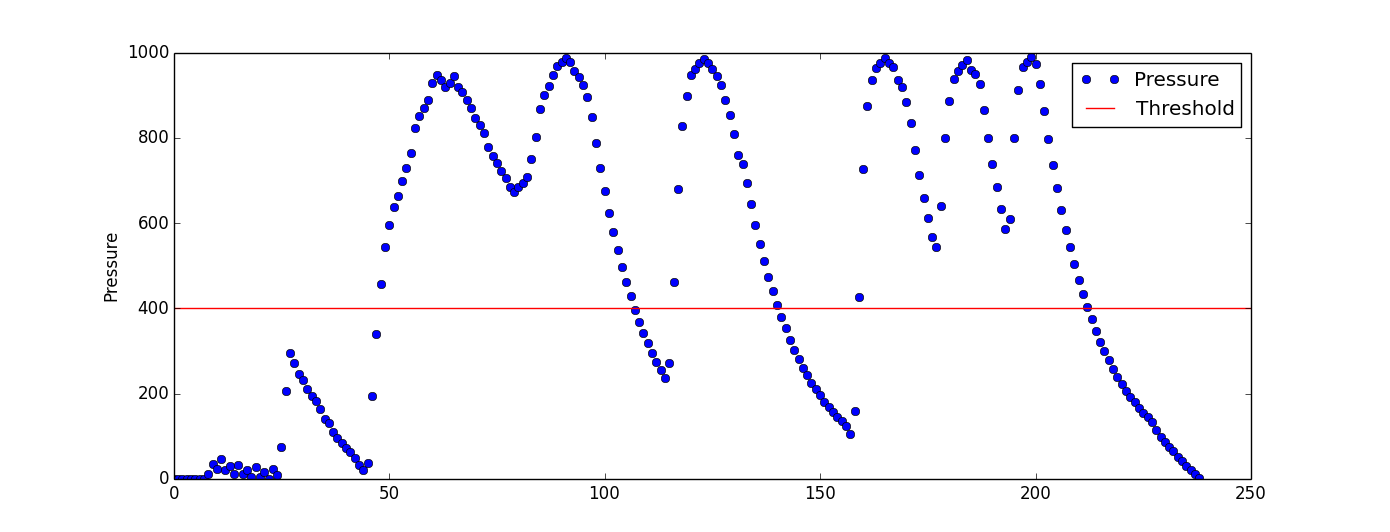
\includegraphics[width=1.0\textwidth]{complexGesture.png}
  \caption{Complex pressure gesture}
  \label{fig:complexGesture}
\end{figure}

\section{Tactons}

To the best of my knowledge, this work is the first to explore dynamic vector-based tactons to exploit haptic cues of edges, corners and directions. The tactons proposed by Pietrzak et al. \cite{pietrzak2009creating} are based on pin arrays. In his paper, it is interesting to note how the designed tactons evolved as user experiments were conducted. The tactons used for the HaptiQ, instead, are merely based on common sense rather than experimentation. Evaluating the current set of tactons and eventually producing a new improved set is part of the future work discussed in the next chapter.

During one of the meetings with Saad, we discussed a subset of the tactons presented in this report. His feedback was positive. The meeting after, when trying the HaptiQ, he was able to decode the behaviours efficiently. This cannot be considered a study of any kind, but his feedback was very valuable to define how the HaptiQ has evolved so far. 

\section{Applications}

The applications presented in this project function as proof of concepts only. Therefore, the applications can be improved largely. The graph visualiser, for example, could support the deletion of haptic objects and the possibility to save and load graphs for later uses. The functions visualiser, instead, can be of great help to students taking courses in mathematics both at school and university level. The application performs very well already, but there are still some issues with scaling and zooming to be solved. 

\section{Summary}

This project was very open-ended and consisted of many different components. Initially, I planned to conduct a user study to evaluate the HaptiQ. However, due to major ethical issues, I decided, with my supervisor, to focus more on the engineering aspects of the HaptiQ and its API. Nonetheless, an iterative process was used rather than a well structured one with well defined requirements. This allowed me to created two devices, with the second one completely re-engineered, and to evolve the API as needed.    

As previously stated, no user study has been conducted to formally evaluate the device.
The project, however, has been assisted and supervised throughout the whole design and implementation phases by Dr Miguel A. Nacenta, who is an expert in Human-Computer Interaction and haptic interfaces. The contribution of Dr Nacenta has been particularly fundamental to validate the design process of the hardware and the tactons.

Conclusions can also be drawn by comparing the device with the state of the art in haptic technology. \\
The HaptiQ, unlike MIMs \cite{brock2010usage} and inFORM \cite{follmer2013inform}, can be used on any interactive surface as long as it is possible to track the device. The HaptiQ, for example, can be used on a normal paper map assuming a top-down tracking mechanism is provided. This makes the HaptiQ more flexible and less expensive, since it can be reused in different scenarios.\\
TeslaTouch \cite{bau2010teslatouch} and REVEL \cite{bau2012revel} allow users to perceive tactile cues extrinsically or intrinsically. Both of these systems allow users to feel texture and to follow lines. The HaptiQ uses a variety of tactons to indicate not only lines, but directions as well. In addition, electrovibration or vibrational mechanical motors can be integrated with the HaptiQ to allow textures to be sensed. \\
UltraHaptics \cite{carter2013ultrahaptics} and AIREAL \cite{sodhi2013aireal} provide haptic feedback in a 3D environment. Accuracy, in these systems, is not constant in space. These solutions, in fact, tend to use tactile feedback for media applications to be used by the visually impaired, rather than by blind people. 

Finally, a brief discussion about the objectives that were not achieved is needed. \\
Initially, one of the secondary objectives was to allow dynamic pointing on the interactive surface. But people with visual disabilities may encounter difficulties on keeping track of the relative position of a dynamic pointer, since no visual feedback can be perceived. Therefore, this objective was discarded. \\
The tertiary objectives included: enabling the haptic device to be used collaboratively and allowing the device to sense textures. 
With the focus of the project being on the tactile cues that the HaptiQ could enhance, I decided to give lower priority to any possible feature that could allow communication between two devices. However, the API can support multiple devices. Thus, clients can implement  collaborative features on top of the API.
On the other hand, the objective of adding the possibility to sense texture was not attempted because the frequency at which the servos, used for this project, work is too low \cite{brown2005first}. A possible alternative could be to add a central static actuator to the devices, similar to the point-reference actuator, which could convey texture information to users via electrovibration \cite{bau2012revel, bau2010teslatouch} or mechanical vibration \footnote{Example of vibration motor for haptic feedback available at \url{http://www.precisionmicrodrives.com/vibrating-vibrator-vibration-motors}. [Online; last checked: 04/04/2014].}.   